\setAuthor{Jaan Kalda}
\setRound{piirkonnavoor}
\setYear{2023}
\setNumber{G 10}
\setDifficulty{10}
\setTopic{TODO}

\prob{Alajaama kaugus}
Maja peakaitsmeni tuuakse elektrivool alajaamast jämeda alumiiniumist juhtmepaari abil, millest üks, nn nulljuhe, on maandatud alajaama juures. Mõlemad juhtmed on ühepikkused ja ühesuguse ristlõike pindalaga $S=\SI{35}{\mm\squared}$. Alumiiniumi eritakistus on $\rho=\SI{2.7e-8}{\ohm\m}$. Tegemist on elektriliini kõige alajaamapoolsema tarbimispunktiga --- elektriliin jätkub järgmiste majapidamiste poole. Maja sees on elektri edasi kandmiseks peenemad sinist ja pruuni värvi juhtmed, mis on peakaitsmes ühendatud alajaamast tulevate juhtmete külge: sinine on ühendatud nulljuhtmega ja pruun võrgupinget kandva nn faasijuhtmega. Peale selle saab peakaitsme juurest alguse sealsamas maandatud rohe-kollane maandusjuhe. Maandamine tagab selle, et juhe omab maapinna elektrilist potentsiaali (kui juhtmes on elektrivool, siis kehtib see vaid maanduspunkti lähedal; maandusjuhtmes voolu ei ole). Et maapind on hea elektrijuht, siis on maapinna potentsiaal kõikjal üks ja sama. 

Kui majas on sisse lülitud  elektriradiaator, siis on maja peakaitsme juures pinge sinise ja kolla-rohelise juhtme vahel $U_1=\SI{30}\V$  ning sinise ja pruuni vahel $U_f=\SI{210}\V$. Radiaatori nominaalpinge on $U_n=\SI{230}\V$ ja nominaalvõimsus on $P_n=\SI 2{\kW}$ (st kui radiaatorile rakendatakse nominaalpinge, siis eraldub radiaatoril nominaalvõimsus). Radiaatori välja lülitamisel väheneb rohe-kollase juhtme ja sinise juhtme vaheline pinge väärtuseni $U_0=\SI{20}\V$. Kui pikk on majast alajaamani viiv juhtmepaar? Eeldage, et nii radiaatorit kui ka elektriliinil paiknevaid teisi tarbijaid võib heas lähenduses vaadelda kui takisteid. Muuhulgas tähendab see, et kuigi võrgus on vahelduvpinge, võib arvutusi teha täpselt samamoodi nagu alalispinge puhul.


\hint

\solu
\begin{center}
    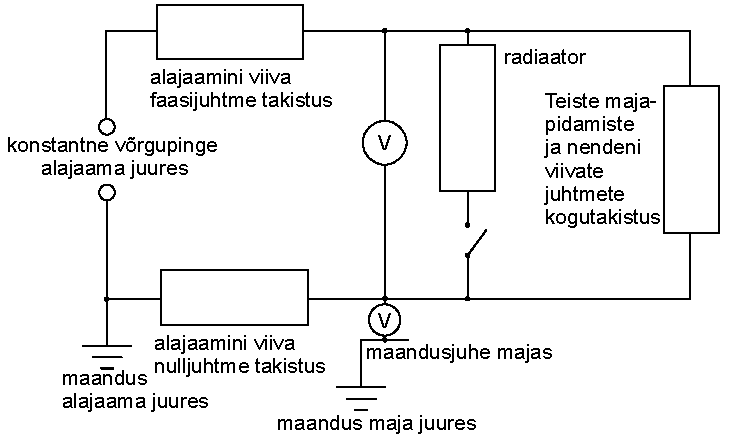
\includegraphics[width=0.8\linewidth]{2023-v2g-10-sol.pdf}
\end{center}

Kõigepealt teeme ekvivalentskeemi: radiaatori (takistusega $R_r$) ja teiste tarbijate (takistusega $R_t$) rööpühendus on järjestikku mõlema juhtmega pingeallika külge, milleks on alajaam; olgu kummagi juhtme takistus $R_j$ ja pinge alajaamas $U_a$. Selles skeemis on teada pinge ühel juhtmel $U_1$ ja pinge radiaatoril $U_f$; kui eemaldada skeemist radiaator, siis tekkiva uue olukorra jaoks on teada uus pinge juhtmel $U_0$. Kummagi ekvivalentskeemi eest saab \p{1}.

Esimesest ekvivalentskeemist saame Kirchoffi pingeseaduse tõttu 
$$U_a=U_f+2U_1;$$
see võrrand annab \p{2} (kui puudub tegur 2, siis \p{1}). 
Teisest ekvivalentskeemist saame tänu Kirchoffi pingeseadusele avaldada uue faasipinge, st pinge teistel koormistel:
$$U_f'=U_a-2U_0=U_f+2(U_1-U_0)=\SI{210}{\V} + 2(30-20)\,\si{\V} = \SI{230}{\V}.$$
see võrrand annab samuti \p{2} (kui puudub tegur 2, siis \p{1}).

Selleks, et leida juhtme pikkus, on meil esimese sammuna vaja leida juhtme takistus. Peale pingete avaldamist on meil on alles jäänud kolm tundmatut takistit, millest radiaatori takistuse saame avaldada tänu nominaalandmetele: 
$$P_n=U_n^2/R_r\;\; \Rightarrow\;\; R_r=U_n^2/P_n=\SI{26.45}{\ohm}.$$
See seos (emb-kumb) annab \p{1}. Kahe tundmatu leidmiseks vajame kahte võrrandit, milleks on Ohmi ja Kirchoffi seadustest tulenev järeldus: jadaühenduses jagunevad pinged võrdeliselt takistustega. Seega
$$U_0/U_f'=R_j/R_t,\quad\p{1}$$
$$U_1/U_f=R_j(1/R_t+1/R_r).\quad\p{1}$$
Lahutades teisest võrrandist esimese saame
$$U_1/U_f-U_0/U_f'=R_j/R_r\Rightarrow R_j=R_r(U_1/U_f-U_0/U_f')=\SI{1.479}{\ohm}.\quad\p{1}$$
Et $R_j=\rho L/S$ \p{1}, siis $L=SR_j/\rho\approx\SI{1920}{\m}$. Numbrilise vastuse eest \p{1}.
\probend